\documentclass[a4paper,oneside,10pt]{scrreprt}

% encoding and locales settings
\usepackage[utf8x]{inputenc}
\usepackage[T1]{fontenc} 
\usepackage[ngerman]{babel}

% package includes for certain purposes
\usepackage{amssymb}   % for symbol \checkmark
\usepackage{booktabs}   % for vertical lines in tables
\usepackage{graphicx}
\usepackage{url}

% style
\usepackage{palatino}   % more beautiful font


% meta information mostly for titlepage
\author{Daniel Böhmer, Tarik Alchanaa, Patrick Nicolaus; IT2007}
\date{28. Juni 2010}
\title{Projekt-Management:\\Pflichtenheft zum Projekt Hotelres 2 \\
    \vspace{2 cm} \includegraphics[width=0.5\textwidth]{logo.png}}


\hyphenation{Pro-dukt-um-ge-bung}

\begin{document}

\maketitle{}

\tableofcontents{}

\sloppy{}


\chapter{Zielbestimmungen}

\section{Musskriterien}

Das bestehende System soll mit Fehlerkorrekturen versehen werden und 
Verbesserungen hinzugefügt werden. Dies sind Optimierungen der 
Benutzerfreundlichkeit und Teile der Wunschkriterien des 
Vorgängerprojekts.

\begin{enumerate}
    \item Buchungssystem
    \begin{itemize}
        \item Zwei Buchungen können sich um 1 Tag überschneiden, so dass 
        ein Gast vormittags auscheckt und der nächste Gast an demselben 
        Tag einchecken kann
    \end{itemize}
    
    \item Login-System
    \begin{itemize}
        \item Die Rechtestufe für Gastkonten (wenig privilegierte 
        Benutzer) soll weiterhin nicht benutzt werden
        \item Für den Gast soll trotzdem ein Zugang zu 
        Informationen über die getätigte Buchung möglich sein
        \item Der Gast soll per E-Mail einen URL mit einer 
        eindeutigen Kennung und einem geheimen Schlüssel (sog. 
        \emph{Token}) bekommen, mit dessen Hilfe die Informationen abgerufen 
        werden können
    \end{itemize}    

    \item Visualisierung
    \begin{itemize}
        \item Übersichten über die Belegungsdichte in einem Zeitraum 
        sollen nicht nur für einen Monat, sondern auch für größere 
        oder kleinere Zeiträume möglich sein
        \item die Belegungsdichte in einem bestimmten Zeitraum soll 
        als visueller Graph dargestellt werden, um Trends einfacher 
        erkennen zu können
    \end{itemize}  

\end{enumerate}


\section{Wunschkriterien}

\begin{enumerate}
\item Rechnung erstellen
\item Zusatzleistungen buchen
\end{enumerate}

\section{Abgrenzungskriterien}
\begin{enumerate}
\item Ein Nutzerhandbuch und eine Online-Hilfe werden vorerst nicht erstellt
\item Eine vollständige Übersetzung ins Englische oder andere 
Sprachen wird vorerst nicht erstellt
\end{enumerate}





\chapter{Produkteinsatz}
\section{Anwendungsbereiche}

Dieses System wird für die Vermietung von touristischen Unterkünften verwendet.


\section{Zielgruppen}

Diese Anwendung ist für Betreiber von touristischen Unterkünften 
gedacht. Dies kann den Bereich von einer einzelnen Ferienwohnung bis zu 
einem großen Hotel umfassen.

\section{Betriebsbedingungen}
Dieses System soll sich bezüglich der Betriebsbedingungen nicht wesentlich von anderen Webanwendungen unterscheiden.

\begin{itemize}
\item Betriebsdauer: täglich, 24 Stunden
\item Die Sicherung der Datenbank muss manuell oder automatisiert vom örtlichen Administrator, dem Händler oder einem externen Dienstleister durchgeführt werden
\item Fehlerhafte Daten können vom Administrator entfernt werden
\end{itemize}






\chapter{Produktumgebung}

Das Produkt ist weitgehend unabhängig vom Betriebssystem, sofern folgende Produktumgebung vorhanden ist.

\section{Software}

\begin{itemize}
\item Client-PCs
    \begin{itemize}
    \item IP-fähiges Betriebssystem
    \item aktueller Browser
        \begin{itemize}
        \item Microsoft Internet Explorer ab Version 7
        \item Mozilla Firefox
        \item Opera
        \end{itemize}
    \item optional: aktiviertes JavaScript für mehr Komfort
    \end{itemize}

\item Server lokal oder mit breitbandiger Verbindung zum Client
    \begin{itemize}
    \item HTTP-Server
    \item für nicht vertrauenswürdige Netzwerke SSL
    \item PHP (mindestens Version 5)
    \item die Grafikbibliothek
    \item MySQL (mindestens Version 4.1)
    \end{itemize}
\end{itemize}

\section{Hardware}

\begin{itemize}
\item Client
    \begin{itemize}
    \item Netzwerkschnittstelle
    \end{itemize}
\item Server
    \begin{itemize}
    \item Netzwerkschnittstelle
    \item ausreichend Kapazität an Primär- und Sekundärspeicher für die genannte Server-Software und das Ausführen der Script-Dateien
    \end{itemize}
\end{itemize}


\section{Orgware}

\begin{itemize}
\item Gewährleistung einer permanenten Netzwerkanbindung
\end{itemize}

\chapter{Produktinformationen}

\section{Benutzerfunktionen}

\begin{itemize}
\item \textbf{/F0010/} Benutzer anmelden:  \\
Der Benutzer meldet sich mit einem Benutzernamen und Passwort am System an. Die Benutzerverwaltung wird vom Administrator durchgeführt. Bei fehlerhaften Eingaben, wird eine Fehlermeldung ausgegeben.

\item \textbf{/F0011/} Benutzer abmelden: \\
Der Benutzer kann sich manuell vom System abmelden. Nach Ablauf eines bestimmten Zeitintervalls wird der angemeldete Benutzer automatisch abgemeldet. 

\item \textbf{/F0020/} Benutzer anlegen:  \\
Der Administrator kann neue Benutzer anlegen und ein Benutzernamen und ein Passwort vergeben.

\item \textbf{/F0021/} Benutzer ändern: \\
Der Administrator kann die Daten eines Benutzers ändern. Er kann den Benutzernamen und das Passwort ändern.

\item \textbf{/F0022/} Benutzer entfernen: \\
Der Administrator kann einen Benutzer entfernen. Dem Benutzer ist es dannn nicht mehr möglich, sich am System anzumelden.
 
\item \textbf{/F0030/} Buchung durchführen: \\
Der Benutzer gibt die Kundendaten und die Buchungsdaten in die Buchungseingabemaske ein und speichert die Daten in einer Datenbank. Jede Buchung wird in der Datenbank gespeichert.

\item \textbf{/F0040/} Daten aktualisieren:  \\
Der Administrator kann Daten der Unterkunft in die Datenbank speichern, die für die Buchung notwendig sind. Dazu gehören z.B. die Zimmernummern, die Zimmeranzahl, die Anzahl der Personen. Diese Daten können jederzeit geändert werden.

\item \textbf{/F0050/} Plan erstellen:  \\
Der Benutzer kann jederzeit einen Plan einsehen, um die Belegung der Unterkünfte überschauen zu können.

\item \textbf{/F0060/} Sprache ändern:  \\
Der Benutzer kann die entsprechende Sprache wählen.
\end{itemize}

\chapter{Produktdaten}
Es sind folgende Daten persistent gespeichert:

\begin{itemize}
\item \textbf{/D0010/} Buchungen (\texttt{bookings}): Die Daten für ein Buchungsvorgang
    \begin{itemize}
    \item Anfangsdatum (\texttt{begin})
    \item Enddatum (\texttt{end})
    \item Kommentar des Benutzers, zum Beispiel Sonderwünsche des Gastes (\texttt{comment})
    \item Anzahl der Personen (\texttt{persons})
    \item Sicherheitsschlüssel für die Benutzerinformationsseite 
            (\texttt{security\_token})
    \end{itemize}

\item \textbf{/D0020/} Gäste (\texttt{guests}): Kundendaten
    \begin{itemize}
    \item Vorname (\texttt{firstname})
    \item Nachname (\texttt{lastname})
    \item Straße (\texttt{street})
    \item Hausnummer (\texttt{number})
    \item Postleitzahl (\texttt{zip})
    \item Wohnort (\texttt{city})
    \item Heimatland (\texttt{country})
    \item Telefon (\texttt{phone})
    \item E-Mail (\texttt{email})
    \end{itemize}

\item \textbf{/D0030/} Räume (\texttt{rooms}): Die Informationen zu einem Objekt der Unterkunft
    \begin{itemize}
    \item Name (\texttt{name})
    \item Maximal unterzubringende Anzahl an Gästen (\texttt{capacity})
    \end{itemize}

\item \textbf{/D0040/} Benutzer (\texttt{users}): Die Daten der Systembenutzer
    \begin{itemize}
    \item Benutzername (\texttt{username})
    \item Passwort (\texttt{password})
    \item Zufallsanteil zur Absicherung des Passworts (\texttt{salt})
    \item Rechte (\texttt{rights})
    \end{itemize}
\end{itemize}


\chapter{Produktleistungen}

\begin{itemize}
\item \textbf{/L0100/} Fehlerbehandlung: \\
Bei fehlerhaften Eingaben des Benutzers wird eine Fehlermeldung angezeigt, um den Benutzer zu informieren und Hinweise zu geben.

\item \textbf{/L0200/} Daten speichern: \\
Alle Daten werden dauerhaft in einer Datenbank gespeichert. Der Administrator sollte regelmäßig eine Sicherung der kompletten Daten erstellen.

\item \textbf{/L0300/} Daten akkumulieren: \\
Gespeicherte Daten werden gesammelt und ausgewertet, so dass Zusammenhänge erkennbar und Informationen visuell erfassbar werden.
\end{itemize}


\chapter{Benutzeroberfläche}

Zur besseren Wiedererkennbarkeit beginnt jede Unterseite mit dem gleichen Kopfteil. Dieser beinhaltet den Titel des Projekts, ein Menü zur Navigation zu den verschiedenen Unterseiten und Schalter zum Wechseln der Sprache.

Das eingebaute Login-System greift auf jeder Unterseite. Ist der Benutzer nicht eingeloggt, erhällt er statt der aufgerufenen Unterseite ein Formular zur Eingabe von Benutzernamen und Passwort.

\section{Allgemeine Seiten}

\subsection*{Startseite}

Die Startseite zeigt den Titel der Web-Anwendung, sowie eine Liste von häufig auftretenden Tätigkeiten. Mit Hilfe dieser Linkliste kann der Benutzer schnell wiederkehrende Aufgaben abarbeiten.

\subsection*{Buchungen anlegen}

Diese Seite besteht zur Hauptsache aus einem Formular, dass alle notwendigen Daten aufnimmt, um einen Gast für eine bestimmte Zeit in der Unterkunft einzumieten. Beim Abschicken erzeugt dieses Formular alle notwendigen Datenbankeinträge.

\subsection*{Belegungspläne einsehen}

Mit diesem Werkzeug kann der Benutzer die Gesamtauslastung über einem Zeitraum oder die Belegung eines einzelnen Raums einsehen.

\subsection*{Buchungsdetails ändern}

Die Seite, die die Details einer einzelnen Buchung anzeigt, dient gleichzeitig dazu, diese zu verändern.


\section{Administrative Seiten}

Die folgenden Seiten sind nur benutzbar, wenn der angemeldete Benutzer die Rechte \texttt{admin} trägt.

\subsection*{Benutzerverwaltung}

Hier können weitere Benutzer angelegt oder vorhandene manipuliert werden. Niemand kann die Rechte seines eigenen Kontos ändern oder das Konto löschen. Dies verhindert eine unerlaubte Rechte-Ausweitung sowie ein ungewolltes Aussperren aus dem System.

\subsection*{Räume anlegen}

Für die Verknüpfung von Buchungen mit einem Raum und der Anzeige der Gesamtauslastung müssen dem Hotelres-System die vorhandenen Räume bekannt sein. Auf dieser Seite werden diese Basisinformationen eingepflegt.


\section{Seiten für Gäste}

\subsection*{Buchungsinformationen}

Ein Gast erhält für jede seiner Buchungen einen eindeutigen URL, der 
ihm Zugriff auf diese Seite gibt. Sie zeigt alle Details für diese 
Buchung und bestätigt dem Gast, dass seine Buchung erfolgreich war.

\subsection*{Kontaktseite}

Bei Rückfragen, Änderungen oder einer Stornierung erhält der Gast 
hier Kontaktdaten wie eine Telefonnummer, um mit dem Betreiber in 
Kontakt zu treten.


\chapter{Qualitätsbestimmungen}

\begin{tabular}{lcccc}

\toprule
                        & Sehr wichtig & Wichtig    & Weniger wichtig & Unwichtig \\
\midrule
Robustheit              & \checkmark   &            &                 & \\
Zuverlässigkeit         & \checkmark   &            &                 & \\
Korrektheit             & \checkmark   &            &                 & \\
Benutzerfreundlichkeit  & \checkmark   &            &                 & \\
Effizienz               & \checkmark   &            &                 & \\
Kompatibilität          &              & \checkmark &                 & \\
Vertrauenswürdigkeit    &              & \checkmark &                 & \\
\bottomrule
\end{tabular}

\vspace{1.5cm}

Gegenüber dem Vorgängerprojekt haben sich die beiden Gewichtigungen 
für Kompatibilität und Benutzerfreundlichkeit verschoben. Im Zuge der 
Verbesserungen dieses Projekts wird eine Erhöhung der 
Benutzerfreundlichkeit angestrebt, die teilweise nur mit Hilfe zusätzlicher 
Programme erreicht werden kann. Um dies möglich zu machen, wurde das 
Kriterium Kompatibilität herabgestuft. Neben der Abhängigkeit von der 
Grafikbibliothek soll die bestehende Kompatibilität erhalten bleiben.


\chapter{Globale Testszenarien und Testfälle}

\begin{itemize}
\item \textbf{/T0010/} Benutzer anmelden: \\
Der Benutzer meldet sich mit einem Benutzernamen und Passwort am System an.

\item \textbf{/T0011/} Benutzer abmelden: \\
Der Benutzer meldet sich manuell vom System ab.

\item \textbf{/T0012/} Benutzer automatisch abmelden: \\
Der Benutzer wartet Zeitintervall ab und das System meldet den Benutzer automatisch ab.

\item \textbf{/T0020/} Benutzer anlegen: \\
Der Administrator legt über die Benutzerseite einen neuen Benutzer an.

\item \textbf{/T0021/} Benutzer ändern: \\
Der Administrator ändert den Benutzernamen und das Passwort eines Benutzers.

\item \textbf{/T0022/} Benutzer entfernen: \\
Der Administrator entfernt einen bestehenden Benutzer aus der Datenbank.

\item \textbf{/T0030/} Buchung durchführen: \\
Der Benutzer führt eine Buchung durch. Er gibt alle notwendigen Daten in die Eingabemaske auf der Buchungsseite ein und führt die Buchung aus.

\item \textbf{/T0040/} Plan erstellen: \\
Der Benutzer erstellt einen Plan.

\item \textbf{/T0041/} Graphen ansehen: \\
Der Benutzer überprüft die Auslastung der Unterkunft in einem 
bestimmten Zeitraum.

\item \textbf{/T0050/} Buchungsdetails einsehen: \\
Ein Gast ruft den per E-Mail erhaltenen URL auf und nimmt Einblick in 
seine Buchung.
\end{itemize}


\chapter{Entwicklungsumgebung}

\section{Software}

Es wird darauf geachtet, dass alle Entwicklungswerkzeuge auch für den gewerblichen Einsatz lizenzkostenfrei oder von vornherein vorhanden sind.

\begin{itemize}
\item Plattform
    \begin{itemize}
    \item GNU/Linux oder Windows XP, Windows Vista, Windows 7
    \end{itemize}

\item Lokaler Webserver (XAMP nur für Windows oder generell lokaler Apache / Lighttpd)
\item PHP-Version ab Version 5
\item die noch auszuwählende Grafikbibliothek
\item Lokaler MySQL-Server ab Version 5
\item Entwicklungswerkzeuge
    \begin{itemize}
    \item PHPmyAdmin für SQL-Einrichtung
    \item beliebiger Texteditor
    \item Git und Tortoise Git für Versionsverwaltung
    \end{itemize}

\item alle genannten in der Produktumgebung genannten Browser
\item The GIMP für Grafikbearbeitung
\end{itemize}

\section{Hardware}

\begin{itemize}
\item Rechner mit Netzwerkschnittstelle
\end{itemize}

\section{Orgware}

\begin{itemize}
\item Netzwerkverbindung
\item GitHub Social Coding\footnote{\url{http://www.github.com}}
\end{itemize}


\chapter{Ergänzungen}

Folgende Abbildungen können sich im Laufe der Entwicklung ändern.

\hspace{2.5 cm} % horizontal space between text and graphics

\begin{figure}[h]
\centering
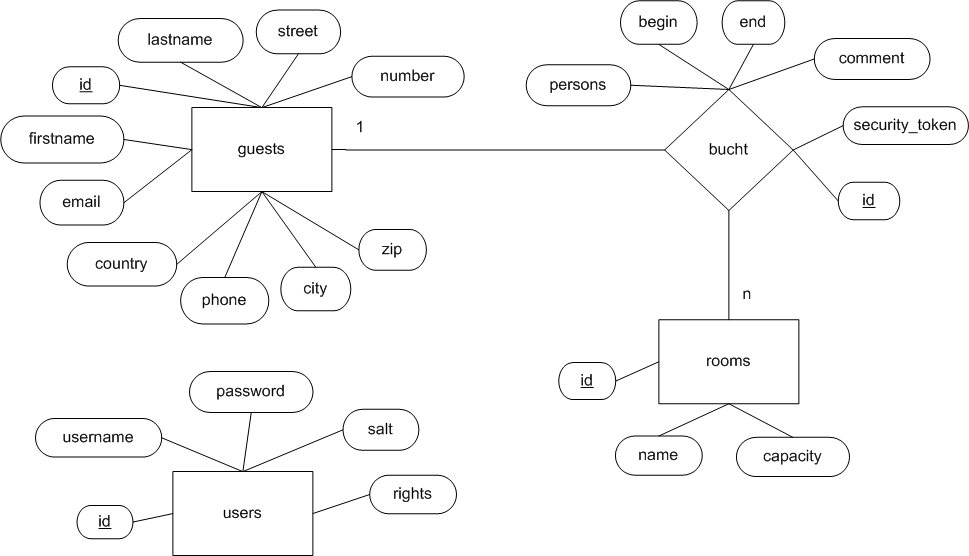
\includegraphics[width=\textwidth]{er-chart.png}
\caption{ER-Diagramm der Datenbank mit den notwendigen Anpassungen}
\label{entity-relationship}
\end{figure}

\begin{figure}[h]
\centering
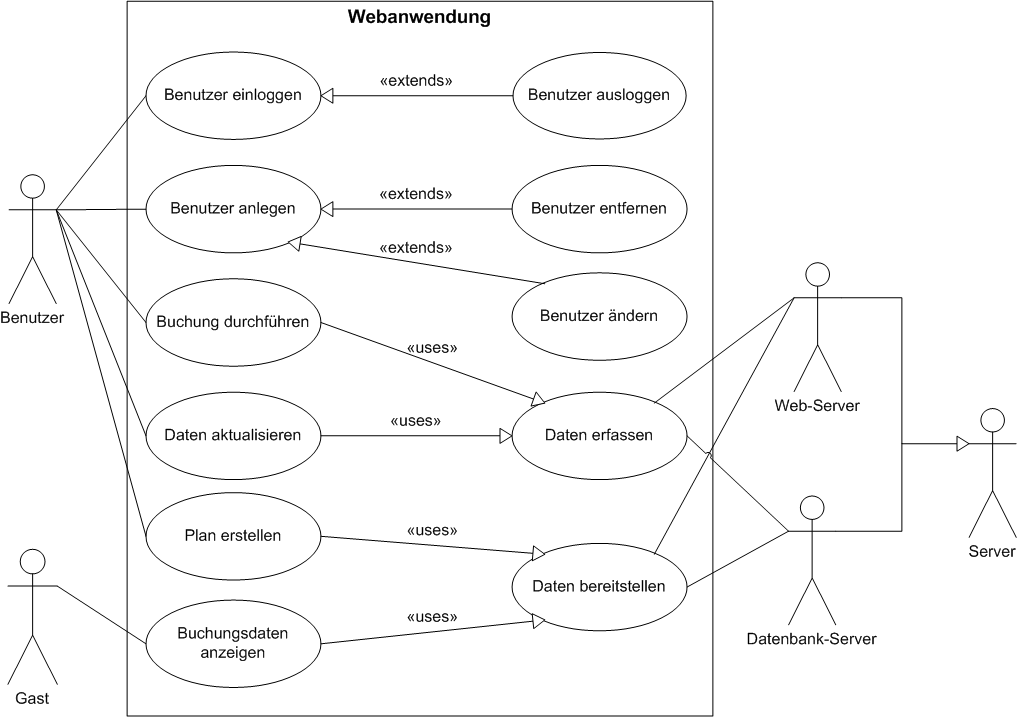
\includegraphics[width=\textwidth]{use-cases.png}
\caption{Use Cases für Hotelres}
\label{use-cases}
\end{figure}




\chapter{Glossar}

\begin{itemize}
\item \emph{Administrator} bezeichnet einen Benutzer mit dem Recht eines Administrators.

\item \emph{Startseite} ist die erste Seite die angezeigt wird, wenn die Anwendung aufgerufen wird. Dazu zählt jedoch nicht der vorgeschaltete Login-Vorgang.

\item \emph{Orgware} sind Rahmenbedingungen in der IT-Projekt-Abwicklung, die weder zu Hardware noch zu Software gehören, jedoch nötig sind, um die Projektziele zu erreichen.
\end{itemize}


\end{document}
